\chapter{Magnetic Induction} \label{chap:MagneticInduction}
Magnetic induction deals with magnetic fields creating electrical voltages or currents through several mechanisms.  

	\section{The Hall Effect}
	\index{Hall Effect}
	The \gls{halleffect} deals with a solid conductor carrying current through a magnetic field.  This causes charge-carrying particles to deflect toward the sides of the conductor, creating a voltage that can be detected.  
	
	
	\section{Lenz's Law}
	
	\gls{lenzslaw} states that in the presence of a changing magnetic field, a current will flow in a loop that generates a magnetic field opposite to the direction of the change.  
	
	
	Several examples are shown below: 
	
	\begin{mdframed}[backgroundcolor=blue!10!white]
		\begin{center}
			
			
			\textbf{Example \thesection.1}	
		\end{center}
		
		\textbf{Problem: }A square of metal is located along the same plane as the page.  A magnetic field is directed into the page, and is getting stronger.  In what direction will current flow?  
		
		\textbf{Solution:} We begin by drawing a diagram:
		
		\begin{center}
			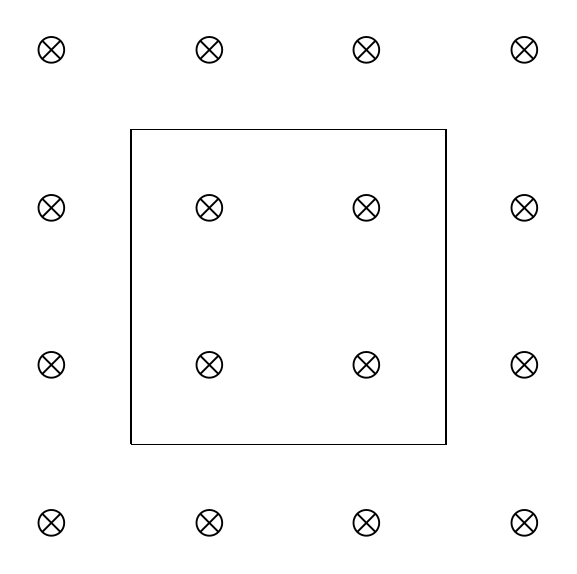
\begin{tikzpicture}
		\draw (0,0) -- (4,0) -- (4,4) -- (0,4) -- (0,0);
		\node at (-1,-1) (nodeS) {$\bigotimes$};
		\node at (-1,1) (nodeS) {$\bigotimes$};		
		\node at (-1,3) (nodeS) {$\bigotimes$};
		\node at (-1,5) (nodeS) {$\bigotimes$};		
		\node at (1,-1) (nodeS) {$\bigotimes$};
		\node at (1,1) (nodeS) {$\bigotimes$};		
		\node at (1,3) (nodeS) {$\bigotimes$};
		\node at (1,5) (nodeS) {$\bigotimes$};			
		\node at (3,-1) (nodeS) {$\bigotimes$};
		\node at (3,1) (nodeS) {$\bigotimes$};		
		\node at (3,3) (nodeS) {$\bigotimes$};
		\node at (3,5) (nodeS) {$\bigotimes$};					
		\node at (5,-1) (nodeS) {$\bigotimes$};
		\node at (5,1) (nodeS) {$\bigotimes$};		
		\node at (5,3) (nodeS) {$\bigotimes$};
		\node at (5,5) (nodeS) {$\bigotimes$};	
				
			\end{tikzpicture}
		\end{center}
		
Since the magnetic field is getting stronger, the current induced will oppose this change by creating a magnetic field directed out of the page (thereby cancelling some of the growing strength).  Using the third right hand rule, current will flow counterclockwise, as shown below: 
	
	
		\begin{center}
		\begin{tikzpicture}
		\draw (0,0) -- (4,0) -- (4,4) -- (0,4) -- (0,0);
	
		\node at (4,2) (nodeS) {$\uparrow$};	
		\node at (2,4) (nodeS) {$\leftarrow$};
		\node at (2,0) (nodeS) {$\rightarrow$};		
		\node at (0,2) (nodeS) {$\downarrow$};				
		
	
		\end{tikzpicture}
	\end{center}

	\end{mdframed}
	
	
	
	
	
	
	
	\section{Faraday's Law}
	\gls{faradayslaw} extends Lenz's Law by giving it a mathematical description:
	
			\begin{mdframed}[backgroundcolor=orange!20!white]
		
		\begin{equation}
		\varepsilon = - \frac{\partial \Phi}{\partial t}
		\label{equation:faradayslaw}
		\end{equation}
	\end{mdframed}	
	
	